\documentclass[11pt,a4paper]{article}
% ------------------------------------------------------------------
%  TP Docker - Containerisation & Orchestration (report)
% ------------------------------------------------------------------
\usepackage[utf8]{inputenc}
\usepackage[T1]{fontenc}
\usepackage{mathpazo}\usepackage{courier}
\usepackage[english]{babel}
\usepackage[a4paper,margin=2.0cm,top=2.2cm,bottom=2.2cm]{geometry}
\usepackage{graphicx}
\usepackage{xcolor}
\usepackage{listings}
\usepackage{booktabs}
\usepackage{tabularx}
\usepackage{fancyhdr}
\usepackage{titlesec}
\usepackage{caption}
\usepackage{enumitem}
\usepackage{float}
\usepackage{needspace}
\usepackage[most]{tcolorbox}
\usepackage[hidelinks]{hyperref}

% ---------- colours ----------
\definecolor{accent}{HTML}{1D63ED}   % Docker blue
\definecolor{ink}{HTML}{1F2933}
\definecolor{soft}{HTML}{F3F6FA}
\definecolor{rule}{HTML}{C9D3E0}
\definecolor{kw}{HTML}{0B57D0}
\definecolor{cm}{HTML}{6B7785}
\definecolor{st}{HTML}{B3261E}

% ---------- headings ----------
\titleformat{\section}{\Large\bfseries\color{accent}}{\thesection}{0.8em}{}[\vspace{-0.6em}\color{rule}\rule{\textwidth}{0.6pt}]
\titleformat{\subsection}{\large\bfseries\color{ink}}{\thesubsection}{0.8em}{}
\titleformat{\subsubsection}{\normalsize\bfseries\color{ink}}{\thesubsubsection}{0.8em}{}
\setlength{\parindent}{0pt}
\setlength{\parskip}{0.45em}

% ---------- header / footer ----------
\pagestyle{fancy}
\fancyhf{}
\fancyhead[L]{\small\color{cm}TP Docker -- Containerisation \& Orchestration}
\fancyhead[R]{\small\color{cm}Lab report}
\fancyfoot[C]{\small\color{cm}\thepage}
\renewcommand{\headrulewidth}{0.4pt}

% ---------- captions ----------
\captionsetup{font=small,labelfont={bf,color=accent}}

% ---------- code listings ----------
\lstdefinestyle{tp}{
  basicstyle=\ttfamily\scriptsize\color{ink},
  backgroundcolor=\color{soft},
  frame=leftline, framerule=2pt, rulecolor=\color{accent},
  xleftmargin=6pt, framexleftmargin=6pt,
  keywordstyle=\color{kw}\bfseries,
  commentstyle=\color{cm}\itshape,
  stringstyle=\color{st},
  showstringspaces=false, breaklines=true, columns=fullflexible,
  numbers=left, numberstyle=\tiny\color{cm}, numbersep=8pt,
  literate={é}{{\'e}}1 {è}{{\`e}}1 {à}{{\`a}}1 {·}{{$\cdot$}}1 {→}{{$\rightarrow$}}1
}
\lstset{style=tp}
\lstdefinelanguage{Dockerfile}{
  morekeywords={FROM,AS,RUN,CMD,ENTRYPOINT,COPY,ADD,ENV,ARG,WORKDIR,USER,EXPOSE,VOLUME,LABEL,HEALTHCHECK},
  sensitive=true, morecomment=[l]{\#}, morestring=[b]"}
\lstdefinelanguage{yaml}{
  morekeywords={services,image,build,ports,volumes,networks,environment,depends_on,command,restart,profiles,name,driver,on,jobs,steps,uses,with,run,needs,runs-on,env,push,branches},
  sensitive=true, morecomment=[l]{\#}, morestring=[b]"}
\lstdefinelanguage{shell}{
  morekeywords={docker,compose,build,run,network,volume,create,inspect,images,ps,rm,push,tag,login,logs,exec,system,prune,curl},
  morecomment=[l]{\#}, morestring=[b]"}

% ---------- boxes ----------
\newtcolorbox{note}[1][]{colback=soft,colframe=accent,boxrule=0.6pt,arc=2pt,
  left=8pt,right=8pt,top=6pt,bottom=6pt,fonttitle=\bfseries\small,title=#1}
\newcommand{\shot}[3][0.74]{%
  \begin{figure}[H]\centering
  \fcolorbox{rule}{white}{\includegraphics[width=#1\textwidth]{screenshots/#2}}
  \caption{#3}\end{figure}}

% ==================================================================
\begin{document}

% ---------------- title page ----------------
\begin{titlepage}
\centering
\vspace*{1.5cm}
{\color{accent}\rule{\textwidth}{1.2pt}}\\[0.8cm]
{\Huge\bfseries\color{ink} Containerisation and\\[0.25cm] Micro-services Orchestration}\\[0.5cm]
{\Large\color{accent} Lab report -- TP1 Docker}\\[0.8cm]
{\color{accent}\rule{\textwidth}{1.2pt}}\\[1.6cm]

\begin{tabular}{l}
\textbf{Students}\\[0.2cm]
Oussema \textsc{Bouchaala}\\
Mouin \textsc{El Dabbabi}\\
Mohamed Amin \textsc{Saddoud}\\
Mohamed Helmi \textsc{Lakhdhar}\\
\end{tabular}\\[1.6cm]

\begin{tabular}{ll}
\textbf{Part A} & Graded Docker tutorial (Spring Boot, MongoDB, Docker Compose)\\
\textbf{Part B} & Visit-Counter: Dockerfile, network, volume, Compose, scaling\\
\textbf{Part C} & CI/CD pipeline (GitHub Actions $\rightarrow$ Docker Hub)\\
\end{tabular}

\vfill
{\large Academic year 2026--2027}\\[0.3cm]
{\small Generated on \today}
\end{titlepage}

\tableofcontents
\newpage

% ==================================================================
\section{Introduction and environment}

The objective of this lab is to master the complete life-cycle of a container: writing an
optimised and secure image, connecting containers through a user-defined network,
persisting data with volumes, orchestrating several services with Docker Compose,
publishing the image on Docker Hub and finally automating the whole chain with a
CI/CD pipeline.

All the work was done on a Windows 11 laptop running \textbf{Docker Desktop 4.43.2}
(Engine 28.3.2, WSL2 back-end). The commands were typed in the integrated terminal of
Docker Desktop (PowerShell); every screenshot of this report is taken from that
real session.

\begin{note}[Project layout]
\footnotesize
\begin{verbatim}
TP_Docker_Bouchaala_ElDabbabi_Saddoud_Lakhdhar/
|-- partA-tutorial/            Part A - Spring Boot apps from the course
|   |-- application-one/       REST API + Dockerfile
|   `-- item-service-mongodb/  Spring Boot + MongoDB + docker-compose.yml
|-- partB-visit-counter/       Part B - Visit-Counter micro-services
|   |-- app/                   app.py, requirements.txt
|   |-- tests/                 unit tests (pytest)
|   |-- nginx/nginx.conf       bonus load balancer
|   |-- Dockerfile  .dockerignore  docker-compose.yml  .env
|-- .github/workflows/ci-cd.yml  Part C - pipeline
`-- report/                    this LaTeX report + screenshots
\end{verbatim}
\end{note}

\subsection*{Part 0 -- Environment check}
\shot{00_docker_version.png}{\texttt{docker version}: client and server (Docker Desktop 4.43.2, Engine 28.3.2) are available.}

% ==================================================================
\section{Part A -- Docker tutorial (Spring Boot, MongoDB, Docker Compose)}

The graded tutorial is the video course \emph{Containerize Spring Boot CRUD App with
Docker and Docker Compose} (Packt). It goes through: why containers, images vs.
containers, Dockerfile, \texttt{docker build}, Docker Hub, running containers,
inter-container communication with a MongoDB database, debugging inside a container
and Docker Compose. We reproduced the two projects of the course in
\texttt{partA-tutorial/}.

\subsection{Key concepts learned}
\begin{description}[leftmargin=1.2em,style=nextline]
  \item[Image vs. container] An \emph{image} is a read-only, layered template (code +
  runtime + libraries + configuration). A \emph{container} is a running instance of an
  image with its own writable layer, process tree, network stack and file system.
  \item[Why Docker] ``It works on my machine'' disappears: the same image runs
  identically on every machine; containers start in seconds, are lighter than VMs
  (they share the host kernel) and are isolated from each other.
  \item[Workflow] \texttt{Dockerfile} $\xrightarrow{\texttt{docker build}}$ image
  $\xrightarrow{\texttt{docker push}}$ registry (Docker Hub)
  $\xrightarrow{\texttt{docker pull / run}}$ container.
  \item[Useful commands] \texttt{docker ps}, \texttt{images}, \texttt{logs},
  \texttt{exec -it <c> sh}, \texttt{rm -f}, \texttt{rmi}, \texttt{tag}, \texttt{push}.
\end{description}

\subsection{Project 1 -- \texttt{application-one} (REST API)}
A minimal Spring Boot 2.5 application exposing \texttt{GET /api/v1/welcome}.
The course Dockerfile was \texttt{FROM openjdk:11 / ADD target/app.jar / ENTRYPOINT}
with the jar built on the host. Because the \texttt{openjdk} images are deprecated
and to remove the dependency on a local JDK/Maven, we wrote a \textbf{multi-stage}
Dockerfile: the first stage compiles the jar with the Maven wrapper, the second stage
only contains a JRE (Alpine) and the jar, and runs as a non-root user.

\lstinputlisting[language=Dockerfile,caption={\texttt{partA-tutorial/application-one/Dockerfile}}]{code/Dockerfile.partA}

Both images were built on the laptop (the Maven dependencies are downloaded inside
the build stage), then the REST API was tested:

\shot{A1_partA_images.png}{Part A: build of the two Spring Boot images (multi-stage) and pull of \texttt{mongo:7} -- 19.4~min on our slow connection.}
\shot{A2_run_application_one.png}{\texttt{docker run -p 8090:8080}: the endpoint \texttt{/api/v1/welcome} answers, \texttt{docker exec \ldots whoami} shows the non-root user \texttt{spring}, \texttt{docker logs} shows the Spring Boot logs.}

As in the course, the image was also tagged and pushed to Docker Hub
(\path{oussemabouchaala/application-one-img:v1}).

\subsection{Project 2 -- \texttt{item-service} with MongoDB and Docker Compose}
A CRUD REST API (\texttt{/api/v1/items}) storing items in MongoDB. In the course
the two containers are linked with the legacy \texttt{--link} option and the database
is reached through \path{host.docker.internal:28000}. With Compose, both services
share a network and the application reaches MongoDB by its service name; the
connection settings of \path{application-local.properties} are overridden with
environment variables (Spring Boot relaxed binding).

\lstinputlisting[language=yaml,caption={\texttt{partA-tutorial/item-service-mongodb/docker-compose.yml}}]{code/compose.partA.yml}

\shot{A3_compose_mongo.png}{\texttt{docker compose up -d}: Compose creates the network, the \texttt{mongo-data} volume, the MongoDB container and the Spring Boot container.}
\shot{A4_crud_mongo.png}{End-to-end test: two \texttt{POST} requests return \texttt{201 Created}, \texttt{GET} lists the items, and \texttt{docker exec \ldots mongosh} proves that the documents are stored in MongoDB.}

% ==================================================================
\section{Part B -- Visit-Counter micro-services}

\subsection{Architecture}
The application is made of two services:
\begin{itemize}[leftmargin=1.3em]
  \item \textbf{web} -- a Python/Flask application served by Gunicorn. On each request it
  increments the Redis key \texttt{hits} and answers
  \emph{``Bonjour ! Cette page a été vue X fois. Je suis le conteneur [ID]''}. The container
  ID is the hostname of the container (Docker sets it to the short container ID).
  \item \textbf{db-service} -- a Redis 7 (Alpine) instance with \emph{append-only file}
  persistence, storing its data in the named volume \texttt{redis-data}.
\end{itemize}
The web service finds Redis by its DNS name \texttt{db-service}, resolved by the embedded
DNS server of the user-defined bridge network \texttt{app-network}.

\lstinputlisting[language=Python,linerange={7-20,40-76},caption={\texttt{app/app.py} -- the web service (the HTML template, lines 21--37, is omitted)}]{code/app.py}

\subsection{Part 1 -- Dockerfile \& isolation}

\lstinputlisting[language=Dockerfile,caption={\texttt{Dockerfile} (commented)}]{code/Dockerfile}

\paragraph{Choice of the base image.}
We use \texttt{python:3.12-alpine}. Alpine Linux is a minimal distribution
(about 7~MB) built on \texttt{musl} and BusyBox. Compared with the alternatives:

\begin{center}
\begin{tabular}{lll}
\toprule
Base image & Approx. size & Comment\\
\midrule
\texttt{python:3.12} (Debian full) & $\approx$ 1 GB & compilers, many tools -- large attack surface\\
\texttt{python:3.12-slim} (Debian) & $\approx$ 130 MB & good compromise, glibc\\
\textbf{\texttt{python:3.12-alpine}} & $\approx$ 50--60 MB & smallest, fewer CVEs, faster pull/push\\
\bottomrule
\end{tabular}
\end{center}

All our dependencies (Flask, redis-py, Gunicorn) are pure-Python wheels, so the usual
drawback of Alpine (no pre-compiled \texttt{manylinux} wheels for C extensions) does not
apply. The final image is \textbf{96.3~MB} as reported by Docker Desktop (uncompressed layers); the compressed image stored on Docker Hub is only \textbf{22.4~MB}.

\paragraph{Security.} A system user \texttt{app} is created and the instruction
\texttt{USER app} drops root privileges: if the application is compromised, the attacker
is an unprivileged user inside the container. The application files are copied with
\texttt{--chown=app:app}. A \texttt{.dockerignore} keeps tests, caches, \texttt{.env}
and \texttt{.git} out of the build context.

\paragraph{Cache optimisation.} \texttt{requirements.txt} is copied and installed
\emph{before} the source code. Docker caches each layer; as long as the dependencies do
not change, the expensive \texttt{pip install} layer is reused and only the last
\texttt{COPY} is rebuilt. This is visible in Figure~\ref{fig:cache2}: after modifying
\texttt{app.py}, steps 2 to 5 are \texttt{CACHED} and only step 6/6 is executed.

\shot{01_build.png}{First \texttt{docker build -t counter-app:1.0 .} -- every layer is built (base image pulled, \texttt{pip install}, \ldots).}
\shot{02_cache_and_images.png}{Second build without any change: all layers come from the cache; \texttt{docker images} shows the size of \texttt{counter-app:1.0} (96.3~MB).}
\begin{figure}[H]\centering
\fcolorbox{rule}{white}{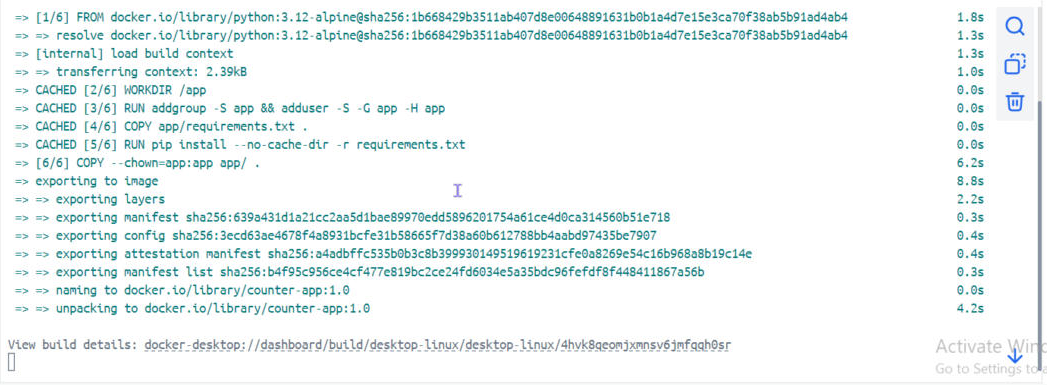
\includegraphics[width=0.95\textwidth]{screenshots/04_cache_code_change.png}}
\caption{Build after a modification of the source code: only the layer \texttt{[6/6] COPY app/} is rebuilt.}\label{fig:cache2}
\end{figure}


\subsection{Part 2 -- Network and volume (manual deployment)}

A user-defined \emph{bridge} network and a named volume are created, then both
containers are started by hand:

\begin{lstlisting}[language=shell]
docker network create app-network
docker volume create redis-data
docker run -d --name db-service --network app-network \
       -v redis-data:/data redis:7-alpine redis-server --appendonly yes
docker run -d --name web-app --network app-network -p 80:5000 counter-app:1.0
\end{lstlisting}

\begin{itemize}[leftmargin=1.3em]
  \item On a \emph{user-defined} bridge, Docker provides an embedded DNS server
  (\texttt{127.0.0.11}): the web container reaches Redis simply with the host name
  \texttt{db-service} (the container name). This does not work on the default
  \texttt{bridge} network, where the deprecated \texttt{--link} option of the course
  would be needed.
  \item Redis is \textbf{not published} on the host (no \texttt{-p}): only containers of
  \texttt{app-network} can reach it -- isolation of the database tier.
  \item \texttt{-p 80:5000} maps port 80 of the host to port 5000 of Gunicorn.
  \item \texttt{--appendonly yes} makes Redis log every write to
  \texttt{/data/appendonly.aof}, i.e.\ inside the volume.
\end{itemize}

\shot{03_manual_run.png}{Creation of \texttt{app-network} and \texttt{redis-data}, pull of \texttt{redis:7-alpine} and start of both containers.}
\shot{05_images_and_ps.png}{\texttt{docker ps}: \texttt{web-app} publishes \texttt{0.0.0.0:80->5000/tcp}, \texttt{db-service} only exposes 6379 internally.}

\begin{figure}[H]\centering
\fcolorbox{rule}{white}{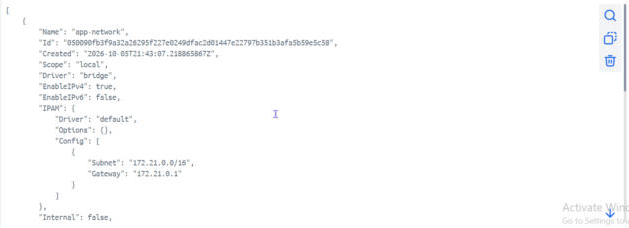
\includegraphics[width=0.48\textwidth]{screenshots/07a_network_inspect.png}}\hfill
\fcolorbox{rule}{white}{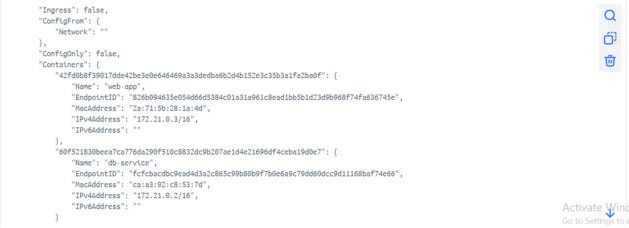
\includegraphics[width=0.48\textwidth]{screenshots/07c_network_containers.png}}
\caption{\texttt{docker network inspect app-network}: bridge driver, subnet 172.21.0.0/16 (left) and the two connected containers \texttt{web-app} (172.21.0.3) and \texttt{db-service} (172.21.0.2) (right).}
\end{figure}

\shot[0.75]{06_browser_manual.png}{The application running in the browser on \texttt{http://localhost/} -- the container ID matches the one of \texttt{web-app}.}

\subsubsection*{Robustness test}
The Redis container is destroyed with \texttt{docker rm -f} and recreated with the same
volume. Because the data lives in \texttt{redis-data} and not in the container's
writable layer, the counter continues where it stopped (8 $\rightarrow$ 9).
The application also retries the Redis connection a few times, so it survives the
restart of its database without being restarted itself.

\shot{08_robustness.png}{Robustness test: the counter keeps its value after \texttt{docker rm -f db-service} and a relaunch on the same volume.}

\subsection{Part 3 -- Orchestration with Docker Compose}

\lstinputlisting[language=yaml,caption={\texttt{docker-compose.yml} (final version)}]{code/docker-compose.yml}
\lstinputlisting[language=shell,caption={\texttt{.env} -- no port is hard-coded in the YAML}]{code/env.txt}

The file centralises the two services, the \texttt{app-network} network, the
\texttt{redis-data} volume and the environment variables. Values such as ports, image
name and Redis host are read from \texttt{.env} through \texttt{\$\{VARIABLE\}}
interpolation. The web service has \textbf{no} \texttt{container\_name}, otherwise it
could not be scaled.\footnote{Compose prints a warning because the volume
\texttt{redis-data} was created manually in Part 2: we deliberately reuse it so the
counter survives the migration from \texttt{docker run} to Compose.}

\subsubsection*{Scaling and analysis}

With a single host port (\texttt{"80:5000"}) the command
\texttt{docker compose up -d --scale web=3} fails:

\shot{09_scale_port_conflict.png}{Three replicas cannot all bind port 80 of the host: \emph{Bind for 0.0.0.0:80 failed: port is already allocated}.}

\paragraph{Why?} A TCP port of the host can be bound by \textbf{only one} process (here
the \texttt{docker-proxy} / port-forwarder of the first replica). When the 2nd and 3rd
replicas try to publish the same host port 80, the kernel refuses the bind. Containers
are isolated in their own network namespaces (each one can listen on 5000
internally), but the \emph{host} side of a port mapping is a shared, unique resource.

\paragraph{Solutions.}
\begin{enumerate}[leftmargin=1.5em]
  \item \textbf{Port range} (what our \texttt{.env} does: \texttt{8081-8083}): each
  replica gets its own host port. It works but the client must know three addresses.
  \item \textbf{Load balancer / reverse proxy} (the real solution): a single entry point
  (Nginx, HAProxy, Traefik) publishes port 80 and forwards each request to one of the
  replicas through the internal network. Docker's DNS resolves the service name
  \texttt{web} to the IPs of all replicas, so the proxy can distribute requests
  (round-robin) and the replicas need no published port at all. In production the same
  role is played by an orchestrator (Docker Swarm routing mesh, Kubernetes
  \texttt{Service}/\texttt{Ingress}) or a cloud load balancer.
\end{enumerate}

\shot{10_compose_up_scale3.png}{\texttt{docker compose up -d --scale web=3} with the port range from \texttt{.env}: network, Redis and three web replicas are started.}
\shot{11_compose_ps_ports.png}{\texttt{docker compose ps}: replicas on ports 8081, 8082, 8083; each one answers with its own container ID while sharing the same counter.}

\paragraph{Bonus -- the load balancer implemented.} We also implemented solution 2:
an \texttt{nginx:alpine} service (Compose profile \texttt{lb}) publishes port 80 and
proxies to \texttt{web:5000}.

\lstinputlisting[caption={\texttt{nginx/nginx.conf}}]{code/nginx.conf}

During the first test all the requests of \texttt{curl} reached the same replica:
nginx runs one worker per CPU and each worker kept its own round-robin pointer, so
every new connection started on the first server. The \texttt{zone} directive puts the
upstream state in shared memory; the requests are then distributed evenly
(Figure~\ref{fig:rr}).

\begin{figure}[H]\centering
\fcolorbox{rule}{white}{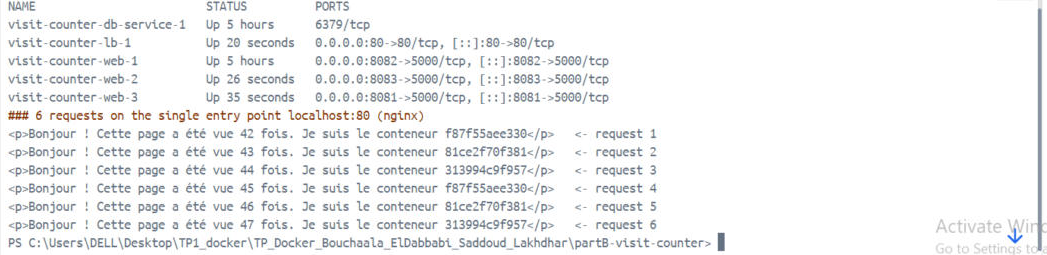
\includegraphics[width=0.95\textwidth]{screenshots/12_lb_round_robin.png}}
\caption{Single entry point \texttt{localhost:80}: the 6 requests are answered in turn by the 3 replicas (\texttt{f87f55aee330}, \texttt{81ce2f70f381}, \texttt{313994c9f957}) and the counter is shared.}\label{fig:rr}
\end{figure}

\begin{figure}[H]\centering
\fcolorbox{rule}{white}{
\includegraphics[width=0.48\textwidth]{screenshots/13a_browser_lb.png}}\hfill
\fcolorbox{rule}{white}{
\includegraphics[width=0.48\textwidth]{screenshots/13b_browser_lb.png}}
\caption{\texttt{docker compose --profile lb up -d --scale web=3}: two consecutive refreshes of \texttt{http://localhost/} are served by two different replicas (\texttt{f87f55aee330}, then \texttt{84c885f319bc}) -- the load balancing works.}
\end{figure}


\subsection{Part 4 -- Publication and cleaning}

\paragraph{Docker Hub.} The image is tagged with the Docker Hub namespace
(\path{<user>/<repository>:<tag>}) and pushed. Docker Desktop was signed in with our
account, so the CLI was already authenticated (\texttt{docker login}).
\begin{lstlisting}[language=shell]
docker tag counter-app:1.0 oussemabouchaala/counter-app:1.0
docker tag counter-app:1.0 oussemabouchaala/counter-app:latest
docker push oussemabouchaala/counter-app:1.0
docker push oussemabouchaala/counter-app:latest
\end{lstlisting}

\shot{14a_tag_push.png}{Tagging and pushing: every layer is uploaded to \texttt{docker.io/oussemabouchaala/counter-app}.}
\shot{14b_push_digest.png}{End of the push: the second tag only re-uses the existing layers (\emph{Layer already exists}) -- both tags point to the same digest.}

\begin{note}[Docker Hub link]
\url{https://hub.docker.com/r/oussemabouchaala/counter-app}\\
\texttt{docker pull oussemabouchaala/counter-app:latest}
\end{note}

\shot[0.6]{15_dockerhub_page.png}{The public repository on Docker Hub.}

\paragraph{Deep clean.} Everything created by the project is removed with
\textbf{one command}:
\begin{lstlisting}[language=shell]
docker compose --profile lb down --rmi all --volumes --remove-orphans
\end{lstlisting}
\texttt{down} stops and deletes the containers and the network, \texttt{--rmi all}
deletes the images used by the services, \texttt{--volumes} deletes the named volume
and \texttt{--remove-orphans} also removes containers of services no longer in the file.

\begin{note}[Why not \texttt{docker system prune -a --volumes}?]
\texttt{docker system prune -a --volumes -f} is the ``industrial'' deep clean: it
deletes \emph{all} stopped containers, unused networks, \emph{all} unused images,
build cache and volumes of the whole machine. On our laptop it would also have
destroyed the data of other projects (Odoo and PostgreSQL volumes\ldots). The
Compose command above is \emph{scoped} to our project, which is the safe choice on a
shared Docker host.
\end{note}

\shot{16a_clean_before.png}{Before: the 5 containers, the network \texttt{app-network} and the volume \texttt{redis-data} of the project.}
\shot{16b_clean_down.png}{The single command stops and removes the containers, then the images (\texttt{nginx:alpine}, \texttt{counter-app:1.0}, \texttt{redis:7-alpine}), the volume and the network.}
\shot{16c_clean_after.png}{After: no container, network, volume or image of the project is left (the image remains available on Docker Hub).}

% ==================================================================
\needspace{12\baselineskip}
\section{Reflection: \texttt{RUN} vs \texttt{CMD}}

\begin{center}
\begin{tabularx}{\textwidth}{lXX}
\toprule
 & \textbf{\texttt{RUN}} & \textbf{\texttt{CMD}}\\
\midrule
When? & At \textbf{build time} (\texttt{docker build}). & At \textbf{run time}, each time a container starts (\texttt{docker run}).\\
Effect & Executes a command and \textbf{commits the result as a new image layer} (installed packages, created users\ldots). & Does not create a layer: it only stores \textbf{metadata} -- the default command of the container.\\
How many? & As many as needed; each one is cached. & Only the \textbf{last} \texttt{CMD} is kept.\\
Override & Cannot be changed when starting a container. & Overridden by the arguments of \texttt{docker run image <cmd>} (or by \texttt{command:} in Compose).\\
Example (ours) & \texttt{RUN pip install -r requirements.txt} & \texttt{CMD ["sh","-c","gunicorn \ldots app:app"]}\\
\bottomrule
\end{tabularx}
\end{center}

In short: \texttt{RUN} \emph{prepares} the image, \texttt{CMD} \emph{says what to launch}
when the image becomes a container. A related instruction is \texttt{ENTRYPOINT}
(used in Part A): it defines the executable that is always run, and \texttt{CMD} then
only provides its default arguments. The \emph{exec form} (JSON array) is preferred
because the process becomes PID~1 and receives the stop signals (\texttt{SIGTERM}) sent
by \texttt{docker stop}.





% ==================================================================
\needspace{12\baselineskip}
\section{Part C -- CI/CD pipeline (GitHub Actions)}

\subsection{Design}
The repository \texttt{OussemaBouchaala/tp-docker-visit-counter} is hosted on GitHub.
We chose \textbf{GitHub Actions} instead of a self-hosted Jenkins: the runners are
provided by GitHub (no server to install), the pipeline is versioned with the code
(\emph{pipeline as code}, like a \texttt{Jenkinsfile}) and the trigger on every commit
is native (\texttt{on: push: branches: [main]}) -- no webhook or SCM polling to configure.

\begin{center}\small
\fbox{\texttt{git push} on \texttt{main}}\\[0.12cm]
$\downarrow$\\[0.05cm]
\fbox{Job 1 -- checkout, Python 3.12, \texttt{pip install}, \texttt{py\_compile}, \texttt{pytest}}\\[0.12cm]
$\downarrow$ \emph{(only if the tests pass: \texttt{needs: build-and-test})}\\[0.05cm]
\fbox{Job 2 -- Docker Hub login, Buildx, build \& push \texttt{:latest} and \texttt{:<commit sha>}}
\end{center}

\begin{itemize}[leftmargin=1.3em]
  \item \textbf{Build and unit tests}: the 4 \texttt{pytest} tests use \texttt{fakeredis},
  an in-memory Redis, so no database is needed in CI. They check the increment of the
  counter, the message format with the container ID, the \texttt{/health} endpoint and
  the HTTP 503 answer when Redis is down. A JUnit report is uploaded as an artifact.
  \item \textbf{Image build and publication}: executed only if the tests pass
  (\texttt{needs}). The credentials are never written in the code: they are stored as
  encrypted repository \emph{secrets} (\texttt{DOCKERHUB\_USERNAME},
  \texttt{DOCKERHUB\_TOKEN} -- an access token, not the password). Each image is tagged
  with \texttt{latest} and with the commit SHA (traceability / rollback), and the
  Buildx layer cache (\texttt{type=gha}) speeds up the next builds.
\end{itemize}

\lstinputlisting[language=yaml,caption={\texttt{.github/workflows/ci-cd.yml}},firstline=10]{code/ci-cd.yml}
\lstinputlisting[language=Python,linerange={11-30},caption={\texttt{tests/test\_app.py} (extract) -- unit tests run by the pipeline}]{code/test_app.py}

\subsection{Results}
The first run (\#1) was triggered by the publication of the repository, \emph{before}
the secrets were created: job~1 (build \& tests) passed, job~2 failed at
\emph{Log in to Docker Hub}. This confirms that no credential is hard-coded and that
the publication job depends on the secrets. After adding them, a new commit on
\texttt{main} (\texttt{523a6db}) triggered run \#2 automatically: both jobs are
green (tests in 9~s, image build and push in 30~s).

\begin{figure}[H]\centering
\fcolorbox{rule}{white}{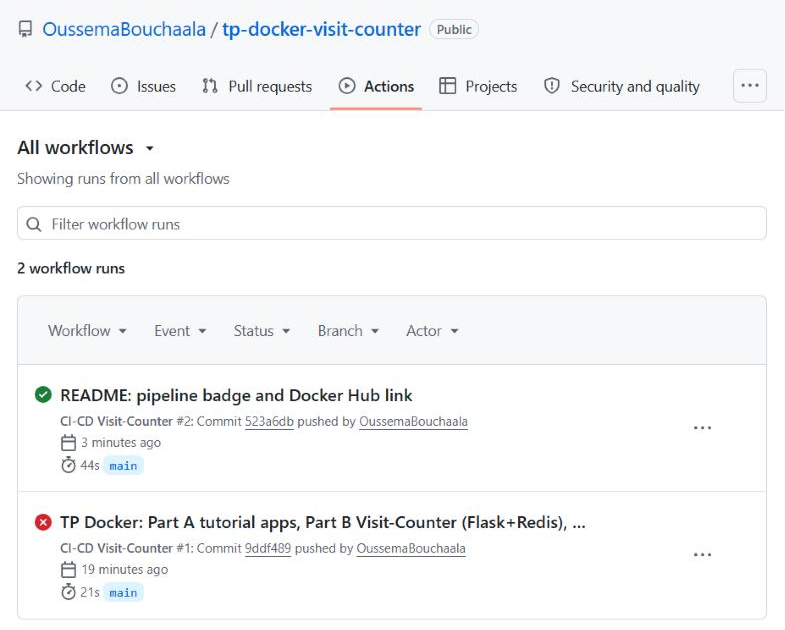
\includegraphics[width=0.48\textwidth]{screenshots/C1_actions_runs.png}}\hfill
\fcolorbox{rule}{white}{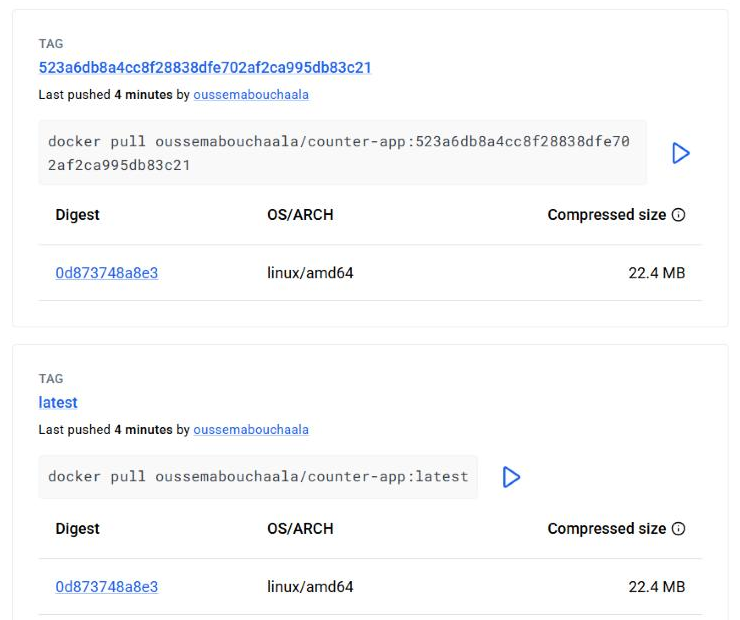
\includegraphics[width=0.48\textwidth]{screenshots/C4_hub_tags_sha.png}}
\caption{Left: the runs triggered by the pushes on \texttt{main} (\#1 without secrets, \#2 successful). Right: Docker Hub receives the image built by the pipeline, tagged with the commit SHA \texttt{523a6db\ldots} and \texttt{latest} (compressed size 22.4~MB).}
\end{figure}

\begin{figure}[H]\centering
\fcolorbox{rule}{white}{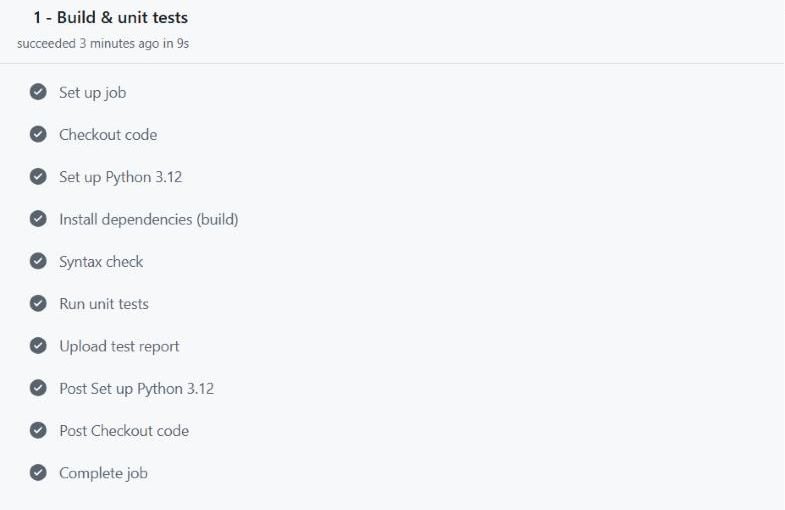
\includegraphics[width=0.48\textwidth]{screenshots/C2_job1.png}}\hfill
\fcolorbox{rule}{white}{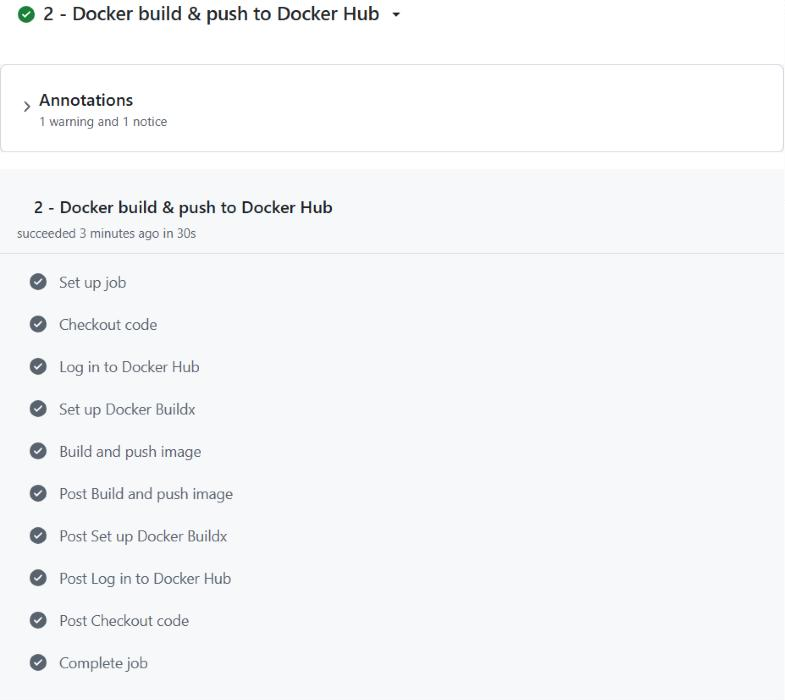
\includegraphics[width=0.48\textwidth]{screenshots/C3_job2.png}}
\caption{Run \#2: job 1 (build, syntax check, unit tests, test report) and job 2 (Docker Hub login, Buildx, build and push) -- all steps successful.}
\end{figure}

\begin{note}[Links]
Repository: \url{https://github.com/OussemaBouchaala/tp-docker-visit-counter}\\
Pipeline: \url{https://github.com/OussemaBouchaala/tp-docker-visit-counter/actions}\\
Image: \url{https://hub.docker.com/r/oussemabouchaala/counter-app}
\end{note}

% ==================================================================
\section{Conclusion}
This lab covered the complete life-cycle of a containerised application. We wrote
small and secure images (Alpine base, non-root user, layer ordering for the cache,
multi-stage build for Java), connected containers through a user-defined network with
DNS-based service discovery, made the data survive the destruction of the container
with a named volume, orchestrated and scaled the services with Docker Compose,
understood why replicas cannot share a host port and solved it with a load balancer,
published the image on Docker Hub, and finally automated tests, build and publication
with a CI/CD pipeline triggered by every commit on \texttt{main}.

\end{document}
